\documentclass[a4paper,10pt]{article}
\usepackage[margin=0.9cm, top=0.7cm, bottom=0.9cm]{geometry}
\usepackage{hyperref}
\usepackage{amsthm}
\usepackage{amsmath}
\usepackage{parskip}
\usepackage{enumitem}
\usepackage{titlesec}
\usepackage{graphicx}
\usepackage{microtype} % optional: better spacing
\usepackage{tikz}
\usepackage{eso-pic}
\linespread{0.95}

\titlespacing*{\section}{0pt}{0.6ex}{0.4ex}

\title{Measuring RNA elongation and splicing speed changes from total RNA-seq}
\author{Jakub Koubele (Beyer lab)}
\date{}
\pagestyle{empty}

\makeatletter
\renewcommand{\maketitle}{
	\begin{center}
		{\LARGE \@title \par}
		\vspace{0.2em} % space between title and author
		{\normalsize \@author}
	\end{center}
	\vspace{0.3em} % space after title block
}
\makeatother

\begin{document}
	
	\maketitle
	
\AddToShipoutPictureFG*{%
	\begin{tikzpicture}[remember picture,overlay]
		% image in the bottom-right corner of the page, inset by your margins
		\node (qr) [anchor=south east]
		at ([xshift=-1.9cm,yshift=0.9cm] current page.south east)
		{
\includegraphics[width=2.2cm]{qr_code.png}};
		% caption under the image
		\node[anchor=north, align=center, font=\footnotesize]
		at ([yshift=-1mm] qr.south) {Link to BioRxiv preprint.};
	\end{tikzpicture}%
}
	
	\textbf{Introduction}
	
	\begin{itemize}[itemsep=0.3em] % reduce vertical spacing between items
		\item Changes in RNA elongation and splicing speed influence the abundance and composition of nascent RNA content.
		\item Total RNA-seq (Ribo-minus) captures both the mature and nascent RNA seq. Elongation and splicing speed changes influence the abundance of intronic reads and their location (coverage), as introns are predominantly present in the nascent RNA.
		\item I am developing a computational method that estimates the log fold changes (LFC) of RNA Pol II elongation speed and the speed of splicing. 
		\item A preprint of this work is available on BioRxiv (link in QR code at the bottom).
	\end{itemize}

\textbf{Elongation speed changes}
\begin{center}
	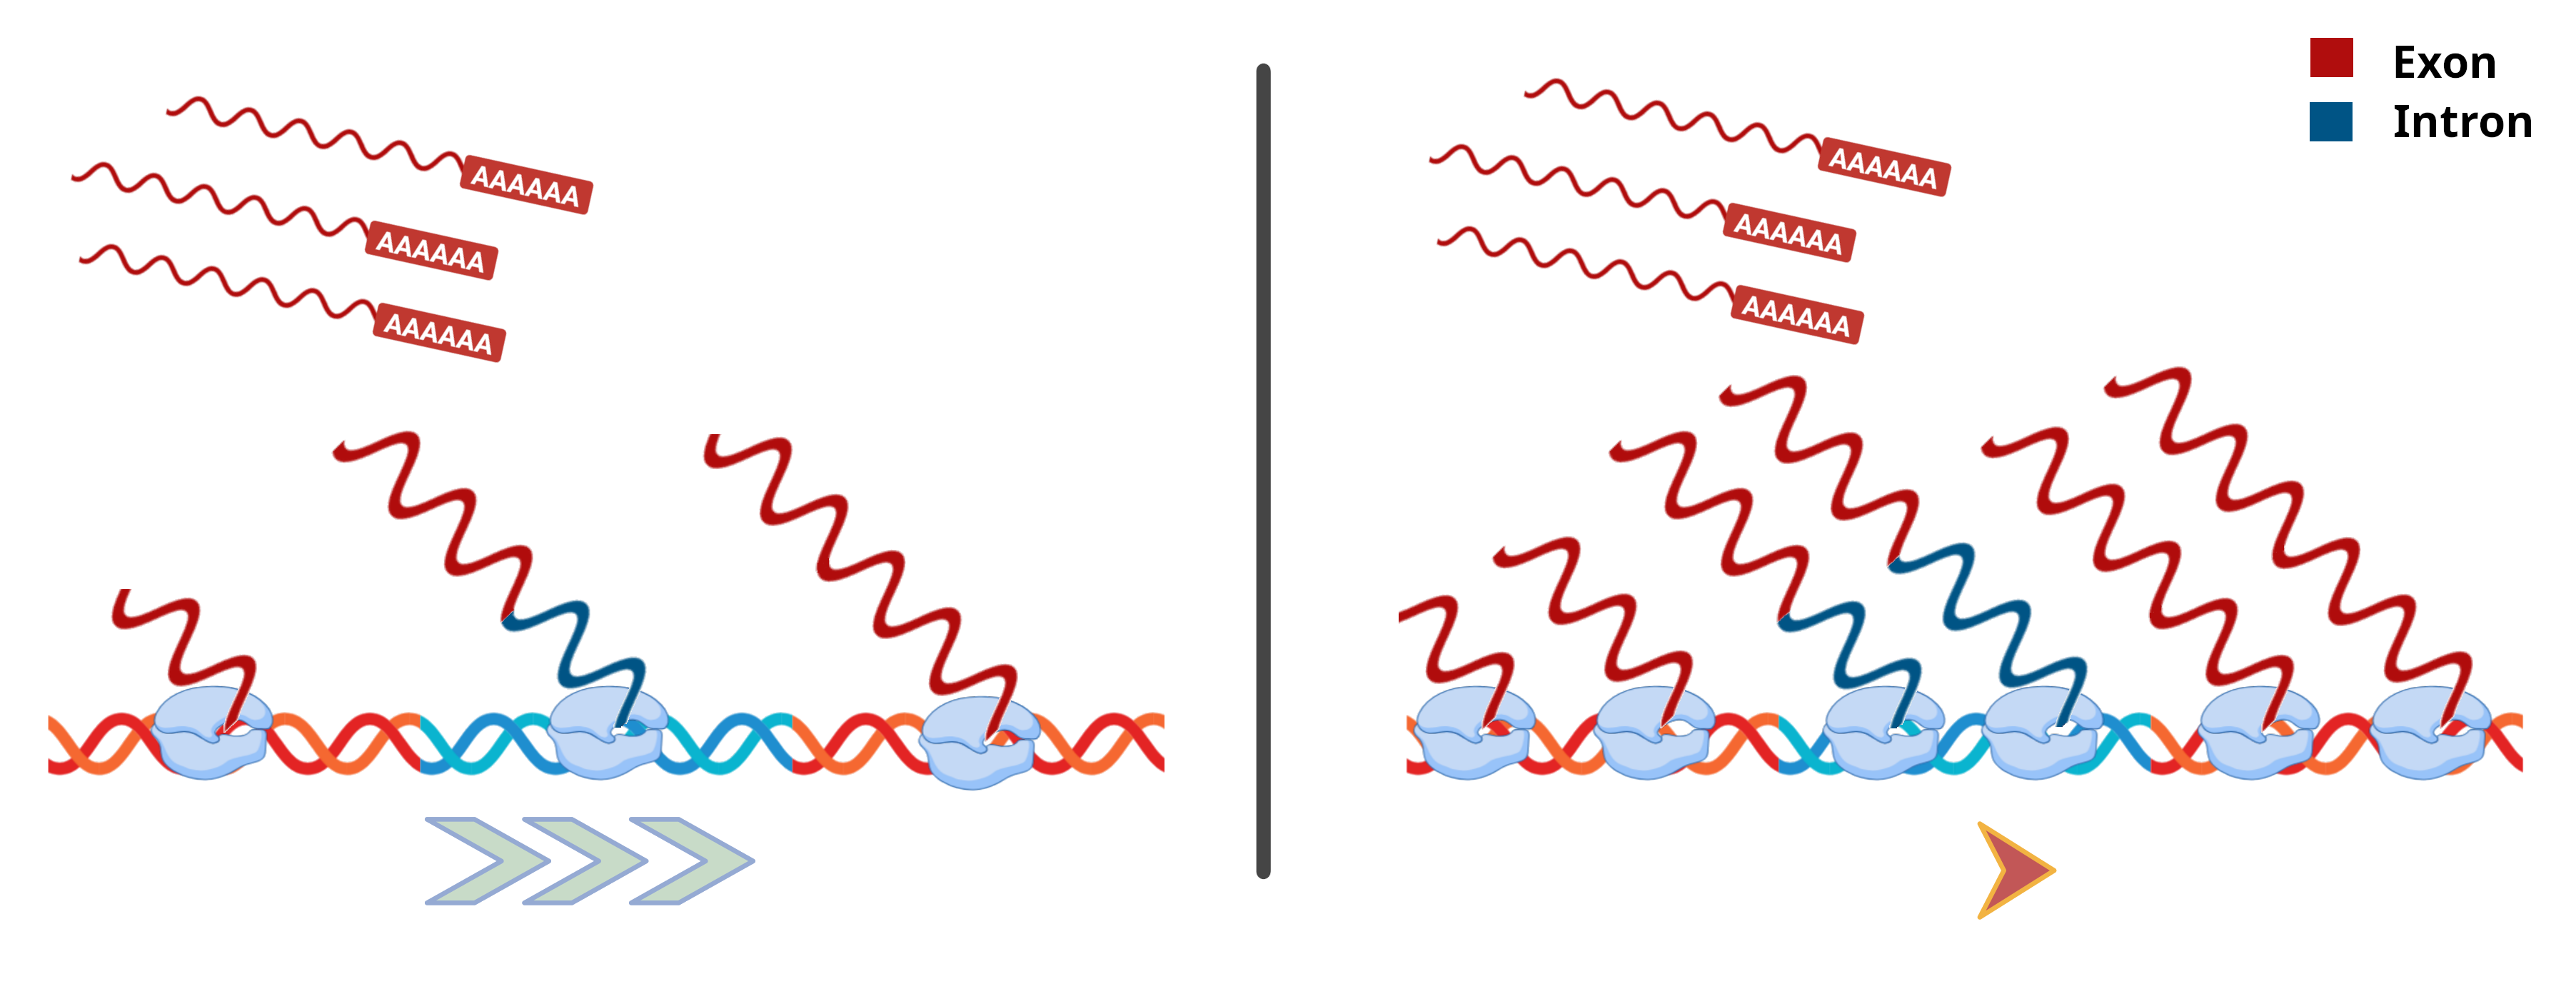
\includegraphics[scale=0.38]{pol_ii_speed_figure_2.png}
\end{center}
\begin{itemize}			
	\item Slower speed $\implies$ higher occupancy of DNA by RNA polymerases $\implies$ more nascent RNA $\implies$ higher fraction of intronic reads.
	
\end{itemize}

\textbf{Splicing speed changes}
\begin{center}
	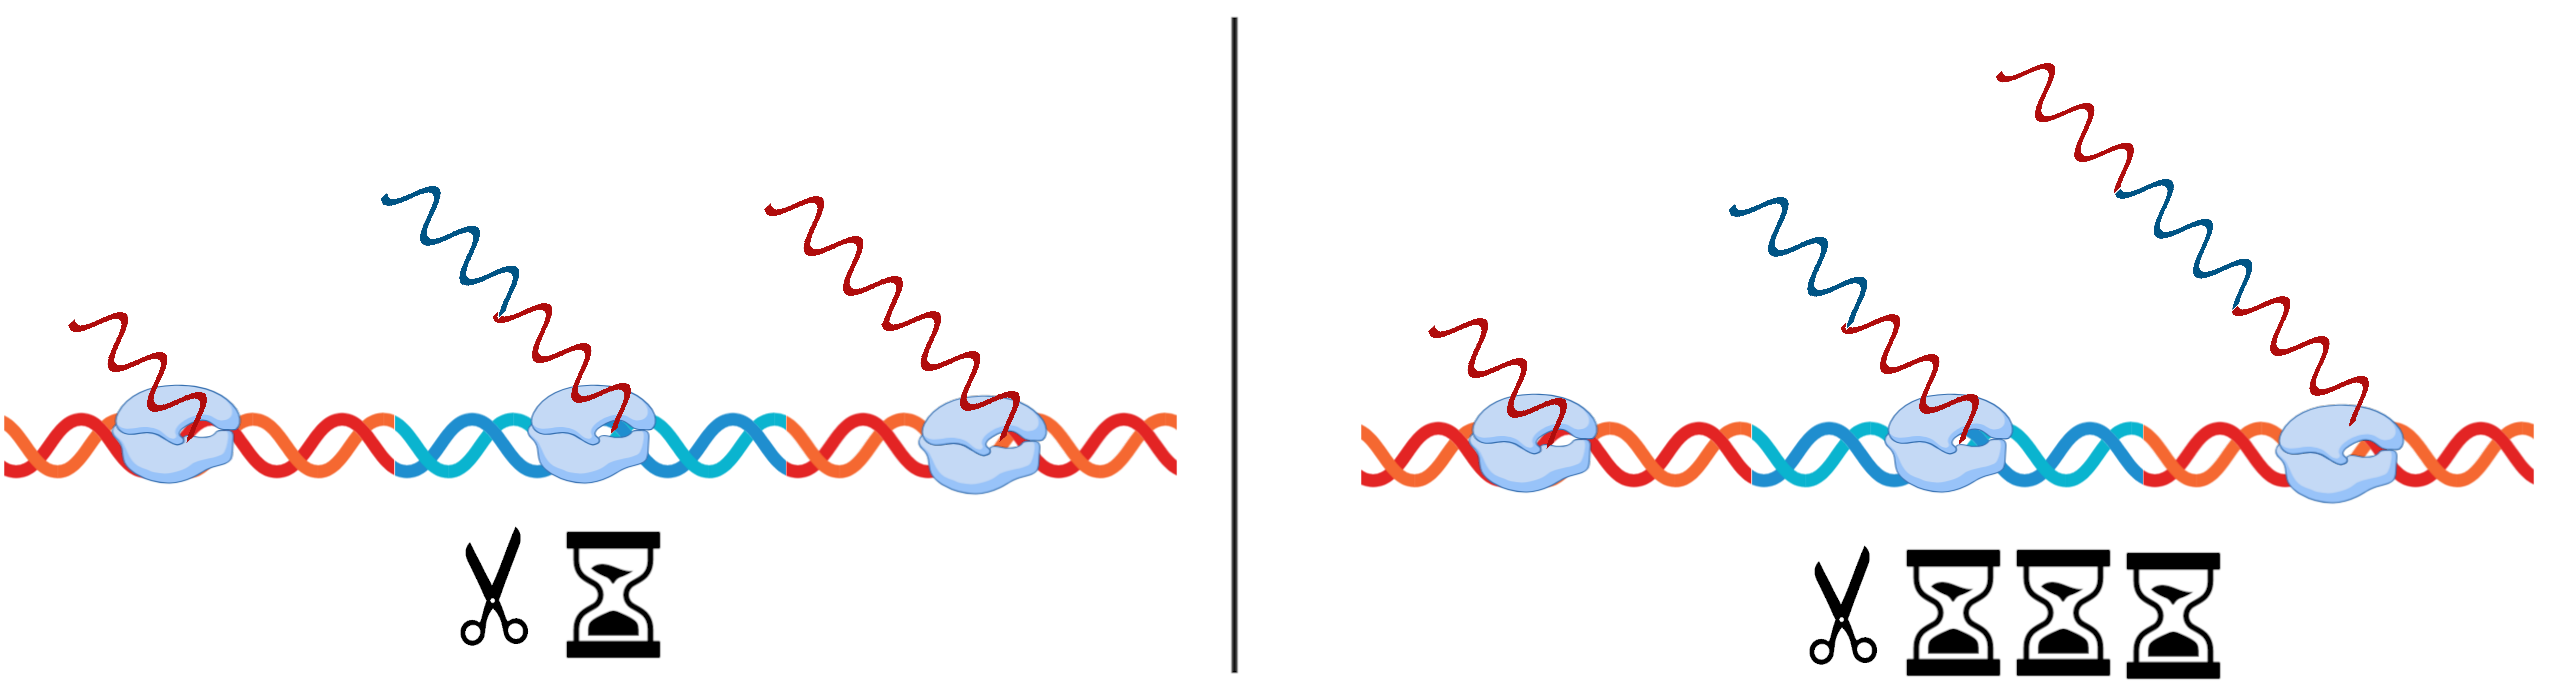
\includegraphics[scale=0.18]{splicing_speed_cropped.png}
\end{center}
\begin{itemize}			
	\item Slower splicing $\implies$ more intronic reads.
	
\end{itemize}

\textbf{Location of intronic reads}


\noindent
\begin{minipage}[t]{0.31\textwidth}
	\vspace{0pt}
	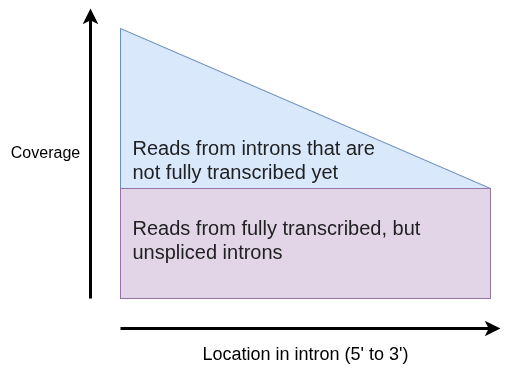
\includegraphics[height=3.75cm, keepaspectratio]{trapezoid.png}
\end{minipage}%
\hfill
\begin{minipage}[t]{0.52\textwidth}
	\vspace{0pt}
	\begin{itemize}\small
	\item Intronic reads come from two sources: 1) from introns that are just being transcribed by Pol II, and 2) from introns that were already transcribed, but not spliced (and degraded) yet.
	\item The amount of Pol II's transcribing intron is inversely proportional to the elongation speed. The amount of fully transcribed but unspliced introns is inversely proportional to the splicing speed.
	\item Thus, the shape of intron coverage depends on the ratio of elongation and splicing speed.
\end{itemize}
\end{minipage}

\textbf{Full model}


\noindent
\begin{minipage}[t]{0.31\textwidth}
	\vspace{0pt}
	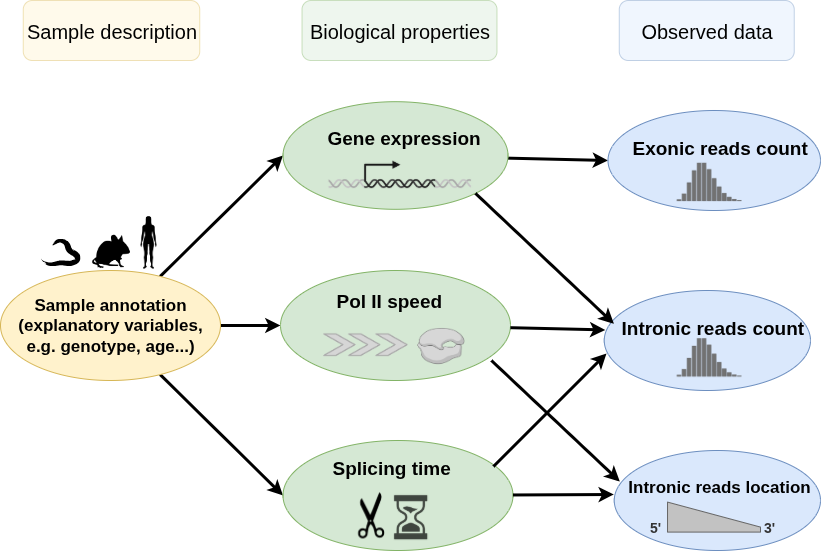
\includegraphics[height=5.90cm, keepaspectratio]{model_final.png}
\end{minipage}%
\hfill
\begin{minipage}[t]{0.52\textwidth}
	\vspace{0pt}
	\begin{itemize}\small
		\item The abundance of exonic and intronic reads, and the location of intronic reads, depend on the LFC of overall gene expression, elongation speed, and splicing speed.
		\item We therefore have a probability model parametrized by these LFC. I fit the model by maximum-likelihood estimation (MLE) on the data.
		\begin{itemize}
			\item[\(\circ\)] Statistical significance (p-values) of LFC can be obtained as well, via Wald test or likelihood-ratio test. 
			
		\end{itemize}
	\end{itemize}
\end{minipage}







	
\end{document}
